\documentclass[11pt]{article}

\usepackage[a4paper, margin=1in]{geometry}
\usepackage{amsmath, amssymb}
\usepackage{algorithm}
\usepackage{algpseudocode}
\usepackage{graphicx}
\usepackage{hyperref}
\usepackage{booktabs}
\usepackage{xcolor}
\usepackage{enumitem}

\hypersetup{colorlinks=true, linkcolor=blue, citecolor=blue, urlcolor=blue}

\begin{document}

% ─────────────────────────────────────────────────────────────────────────
% TITLE PAGE
% ─────────────────────────────────────────────────────────────────────────
\begin{titlepage}
\begin{center}
\vspace*{3.5cm}

{\Huge \textbf{Sublinear MPC Minimum}}\\[0.2cm]
{\Huge \textbf{Spanning Tree}}\\[0.5cm]
{\Large \textit{Implementation, Verification, and Empirical Sublinearity Study}}\\[0.8cm]

{\large Independent Study --- Work Report}\\[1.5cm]

{\large Sriram Metla}\\[0.3cm]
{\large May 2026}\\[2.0cm]

\textbf{\Large International Institute of Information Technology}\\[0.2cm]
\textbf{\large Hyderabad}\\[1.0cm]
\end{center}
\thispagestyle{empty}
\end{titlepage}

\setcounter{page}{1}

% ─────────────────────────────────────────────────────────────────────────
% 1. BACKGROUND
% ─────────────────────────────────────────────────────────────────────────
\section{Background}

The Minimum Spanning Tree (MST) problem on a connected weighted graph
$G = (V, E, w)$ asks for a subset $T \subseteq E$ that spans all vertices and
minimizes $\sum_{e \in T} w(e)$. In the distributed setting the graph is too
large for one machine, so the question becomes how to partition it across many
machines and solve in few rounds of communication.

\subsection{The MPC model}

The Massively Parallel Computing (MPC) model is parameterised by:
\begin{itemize}[topsep=2pt, itemsep=2pt, leftmargin=*]
    \item $n = |V|$, $m = |E|$, with input size $N = m$.
    \item $M$: number of machines.
    \item $S$: words of memory per machine. A \textit{word} is one
          $O(\log N)$-bit unit (one integer ID, one weight, etc.).
\end{itemize}

Each machine has three per-round budgets:

\smallskip
\noindent
\textbf{memory limit} ($S$ words): the maximum data a machine may store at any
moment.

\smallskip
\noindent
\textbf{send limit}: the maximum words a machine may emit in one round
(messages it puts on the wire).

\smallskip
\noindent
\textbf{recv limit}: the maximum words a machine may receive in one round
(messages delivered to its inbox).

\smallskip
The classical MPC model uses $S$ for all three. We allow slightly more
generous \textit{constants} on send/recv at upper levels ($10 \cdot S$ recv,
$20 \cdot S$ send) to make the simulator easier to instrument, but every
limit is strictly $O(S)$ --- linear in the per-machine memory and sublinear
in $n$. Section~\ref{sec:algo} details the actual constants.

The total memory across machines is required to be $M \cdot S = \Theta(N)$.
Algorithm complexity is measured in \textit{rounds} of communication, not
local work.

\paragraph{Memory regimes.} For graph problems:
\begin{itemize}[topsep=2pt, itemsep=2pt, leftmargin=*]
    \item \textit{Strongly super-linear:} $S = n^{1+\varepsilon}$, $O(1)$-round
          algorithms by filtering.
    \item \textit{Near-linear:} $S = \tilde{O}(n)$, $O(1)$-round algorithms
          by graph sketching.
    \item \textit{Strongly sub-linear:} $S = n^{\alpha}$ for
          $\alpha \in (0,1)$. \textbf{This regime is the focus of this work.}
          Algorithms need $O(\log n)$ rounds and a careful tree-of-machines
          structure.
\end{itemize}
We use $\alpha$ for the \textit{memory exponent}, with
$S = \lfloor n^{\alpha} \rfloor$.

\subsection{Bor\r{u}vka's algorithm and the GHS coloring trick}

A \textit{fragment} is a connected vertex subset already known to belong to
the MST. Initially every vertex is its own fragment.

Each Bor\r{u}vka phase:
\begin{enumerate}[topsep=2pt, itemsep=2pt, leftmargin=*]
    \item For each fragment $F$, find its \textit{minimum outgoing edge}
          (MOE) --- the lightest edge with one endpoint in $F$ and one outside.
    \item Add some of these MOEs to the MST, merging fragments.
\end{enumerate}

\textbf{Property 1 (Cut property).} The MOE of any MST fragment belongs to
some MST.

\textbf{Property 2 (Uniqueness).} If all edge weights are distinct, the MST
is unique.

If every fragment merged greedily via its MOE, two fragments that are each
other's MOE would create a cycle. The Gallager--Humblet--Spira (GHS) trick
avoids cycles by \textit{red/blue coloring}:
\begin{itemize}[topsep=2pt, itemsep=2pt, leftmargin=*]
    \item Each fragment is independently colored $\textsc{red}$ or
          $\textsc{blue}$ with probability $1/2$, via shared randomness.
    \item Fragment $F$ merges into $F'$ via MOE $e$ \textbf{only if} $F$ is
          $\textsc{red}$ and $F'$ is $\textsc{blue}$.
\end{itemize}
On expectation $1/4$ of fragments merge per phase, so fragment count shrinks
by a factor of $4/3$ each phase, giving $\log_{4/3}(n) \approx 2.41 \log_2 n$
phases.

\subsection{Machine layout in the sublinear regime}

The $M$ machines are arranged into $L$ \textit{levels}. Level 1 (the
\textit{bottom}) holds the input edges; levels 2 through $L$ are aggregation
layers, transient and rebuilt every phase.

\begin{itemize}[topsep=2pt, itemsep=2pt, leftmargin=*]
    \item Machines per level: $M = \lceil 5m/S \rceil$. (The paper writes
          $4m/S$; we use $5m/S$ because each stored edge takes $5$ words:
          $u$, $v$, $w$, $\textsf{fid}_u$, $\textsf{fid}_v$.)
    \item $R(x, l)$: number of machines at level $l$ responsible for
          fragment $x$.
    \item Branching factor $b = S/4$. Then $R(x, l) = m / b^l$ for
          $l \ge 2$, forced to $1$ at the top.
    \item Tree depth $L = \lceil \log_{S/4}(m) \rceil$.
\end{itemize}

\subsection{The data-driven L1 invariant}

\paragraph{Definition.} A Level-1 machine $\mu$ is \textit{responsible} for
fragment $x$ iff it stores at least one edge incident to $x$.

\paragraph{Lemma.} Let $N_1$ be the total count of (L1-machine, fragment)
responsibility pairs in one phase. Then $N_1 \le 2m$, with equality in Phase 1.

\paragraph{Proof.} Each stored edge $e = (u, v)$ contributes at most two
(machine, fragment) responsibility pairs at its storing machine
(one for $\textsf{fid}_u$, one for $\textsf{fid}_v$). Summing over $m$ edges
gives $N_1 \le 2m$. In Phase 1 every vertex is its own fragment so
$\textsf{fid}_u \ne \textsf{fid}_v$ always, and the bound is tight.

\paragraph{Consequence.} Each Level-1 machine sends one MOE message per
fragment it is responsible for, so the total $L_1 \to L_2$ messages is
exactly $N_1 \le 2m$. Each message is $5$ words, so the average recv at L2
is
\[
    \frac{N_1 \cdot 5}{M} = \frac{2m \cdot 5}{5m/S} = 2 \cdot S
    \quad \text{words per machine.}
\]
This bound is independent of $\alpha$, of $n$, and of the random tree
construction. It is the foundation of strict sublinearity in our simulator.

\subsection{Chernoff bounds}
\label{sec:chernoff}

The data-driven invariant bounds the \textit{average} load. To bound the
\textit{maximum} we use Chernoff inequalities, because each Level-1 machine
picks its parent at Level 2 uniformly at random.

\paragraph{Setting.} Let $X_1, \ldots, X_k$ be \textit{independent}
$0/1$-valued (Bernoulli) random variables. Their sum $X = \sum_i X_i$ counts
how many are $1$. Let $\mu = \mathbb{E}[X]$ be its expectation.

\paragraph{Chernoff bound (upper tail).} For any $\delta > 0$,
\[
    \Pr\bigl[X \ge (1+\delta)\mu\bigr] \le
    \begin{cases}
        \exp(-\mu \delta^2 / 3), & 0 < \delta \le 1, \\[4pt]
        \exp(-\mu \delta / 3),   & \delta > 1.
    \end{cases}
\]
The probability that $X$ exceeds its expectation by a factor $(1 + \delta)$
drops exponentially in $\mu \cdot \delta^2$. Large $\mu$ implies tight
concentration.

\paragraph{High-probability bound.} A statement holds \textit{with high
probability} (w.h.p.) if its failure probability is $\le 1/n^c$ for some
constant $c \ge 1$. Setting the Chernoff bound to $1/n^c$ and solving for
$\delta$:
\[
    \mu \cdot \delta^2 \ge 3c \cdot \ln n
    \quad\Longleftrightarrow\quad
    \delta \ge \sqrt{\frac{3c \ln n}{\mu}}.
\]
Two regimes:
\begin{itemize}[topsep=2pt, itemsep=2pt, leftmargin=*]
    \item \textit{Large $\mu$ (large $S$):} $\delta$ is small;
          $X \le (1 + o(1)) \mu$ w.h.p.
    \item \textit{Small $\mu$ (small $S$):} $\delta$ must be large;
          $X \le O(\mu \sqrt{\log n})$ w.h.p.\ at best.
\end{itemize}

\paragraph{Application to L2 fan-in.} The recv at one L2 machine is
$X = \sum_j \mathbb{1}[\text{message }j\text{ lands here}]$, with
$\mu = N_1 / M \le 2S$. Chernoff gives max $\le (1 + \delta) \cdot \mu$
w.h.p.

At our smallest test point ($n = 100$, $\alpha = 0.3$, $S = 5$, $\mu = 10$
words), Chernoff with $\delta = 3$ predicts max $\le 4 \mu = 8 \cdot S$;
we observe $9 \cdot S$. At the largest ($S = 10000$, $\mu = 20000$ words),
Chernoff with $\delta = 0.1$ predicts max $\le 1.1 \cdot 2 S$; we observe
$2.15 \cdot S$.

\paragraph{Where the paper's bound is loose.} The exercise sheet
\cite{exercise12} claims indegree $\le S/2$ at every level $i \ge 2$,
under conditions $\alpha > 1/2$ and (footnote) $S \ge 16$. We work below
those thresholds ($\alpha = 0.3$, $S = 5$) and observe maxima up to
$9 \cdot S$. The asymptotic claim $O(S)$ holds; the constant $1/2$ does not.

% ─────────────────────────────────────────────────────────────────────────
% 2. THE ALGORITHM
% ─────────────────────────────────────────────────────────────────────────
\section{The Algorithm}
\label{sec:algo}

One Bor\r{u}vka phase consists of six steps. Communication steps are 2, 5,
and 6; steps 1, 3, 4 are local.

\paragraph{Round count per phase.} Let $k = \max(2, \lfloor S/4 \rfloor)$.
\[
    \text{rounds per phase} = \underbrace{(L - 1)}_{\text{Step 2 (upward)}}
    + \underbrace{1}_{\text{Step 5 (top}\to\text{L1)}}
    + \underbrace{2 \lceil \log_k(M) \rceil}_{\text{Step 6 (termination)}}.
\]
Multiplying by $\log_{4/3}(n)$ phases gives $O(\log n / \alpha)$ total
rounds.

\paragraph{Per-machine limits used in the simulator.}
\begin{center}
\begin{tabular}{lll}
\toprule
Resource & Level 1 & Levels 2 to $L$ \\
\midrule
Memory & $S$ words (hard) & $20 \cdot S$ words (hard) \\
Recv per round & $10 \cdot S$ words & $10 \cdot S$ words \\
Send per round & $2 \cdot S$ words & $20 \cdot S$ words \\
\bottomrule
\end{tabular}
\end{center}
A \textit{hard} limit raises an exception on violation. If recv would exceed
the recv limit, delivery is split into multiple \textit{sub-rounds} (each
itself a physical round), preserving the per-round bandwidth contract at
the cost of one extra round per split.

\subsection{Step 1: L1 local MOE}

Each L1 machine $\mu$ reads its $\le S/5$ stored edges and computes, for
each fragment $x$ it is responsible for, the minimum-weight edge
$(u, v, w)$ with $u \in x$ and $v \notin x$. No communication.

\subsection{Step 2: Upward aggregation}

\begin{algorithm}[h]
\caption{Upward MOE aggregation}
\label{alg:upward}
\begin{algorithmic}[1]
\For{each L1 machine $\mu$, each fragment $x$ stored at $\mu$}
    \State send the MOE of $x$ at $\mu$ to $\text{parent}(\mu, x, 1)$
\EndFor
\For{level $l \gets 2, \ldots, L$}
    \For{each machine $\mu$ at level $l$ that received any message}
        \State aggregate incoming messages by fragment, keeping
               the min-weight per fragment
        \If{$l < L$}
            \State forward each entry to its parent at level $l + 1$
        \EndIf
    \EndFor
\EndFor
\end{algorithmic}
\end{algorithm}

\subsection{Step 3: Red/blue decisions}

At the top level, each machine independently colors each fragment $x$ it
holds $\textsc{red}$ or $\textsc{blue}$ (shared randomness). If $x$ is
$\textsc{red}$ and its MOE leads to a $\textsc{blue}$ neighbour, record a
merge: $\textsf{merge}[x] = (\text{old\_fid}, \text{new\_fid}, u, v, w)$.

\subsection{Step 5: Direct top \texorpdfstring{$\to$}{->} L1 delivery}

Instead of routing decisions through the tree (paper's approach), we send
them directly from each top-level machine to the L1 machines responsible
for the affected fragment, in one round.

\begin{algorithm}[h]
\caption{Direct top-to-L1 decision delivery}
\label{alg:downward}
\begin{algorithmic}[1]
\For{each top-level machine $\mu$, each fragment $x$ it owns}
    \State $\textsf{recipients} \gets$ L1 machines responsible for $x$
    \For{each $\mu' \in \textsf{recipients}$}
        \If{$x \in \textsf{merge}$}
            \State send $(\text{old\_fid}, \text{new\_fid}, u, v, w)$ to $\mu'$
        \Else
            \State send $(\text{old\_fid}, \textsc{no\_merge})$ to $\mu'$
        \EndIf
    \EndFor
\EndFor
\State \Comment{1 round of communication}
\For{each L1 machine $\mu'$, each decision received}
    \State relabel fids: $\text{old\_fid} \to \text{new\_fid}$
    \State mark $(u, v, w)$ as MST edge
\EndFor
\end{algorithmic}
\end{algorithm}

Total messages $= N_1 \le 2m$, so the per-L1-machine recv is again
$2 \cdot S$ words on average.

\subsection{Step 6: Distributed termination}

The phase loop must know whether more than one fragment survives. Each
top-level machine first counts its locally-surviving fragments
$c_\mu$. A step-doubling $k$-ary reduction ($k = \max(2, \lfloor S/4 \rfloor)$)
sums these to machine $(L_\text{top}, 0)$, then broadcasts the result back.

\begin{algorithm}[h]
\caption{Step-doubling $k$-ary distributed termination}
\label{alg:termination}
\begin{algorithmic}[1]
\State each top-level machine $\mu$ sets $\textsf{partial}_\mu \gets c_\mu$
\State $\textsf{step} \gets 1$
\While{$\textsf{step} < M$} \Comment{upward sum}
    \For{$j \gets 0, k \cdot \textsf{step}, 2k \cdot \textsf{step}, \ldots$}
        \For{$i \gets 1, \ldots, k - 1$}
            \State machine $(L_\text{top}, j + i \cdot \textsf{step})$
                   sends $\textsf{partial}$ to $(L_\text{top}, j)$
        \EndFor
    \EndFor
    \State each receiver adds incoming to its $\textsf{partial}$
    \State $\textsf{step} \gets \textsf{step} \cdot k$
\EndWhile
\State $f_\text{new} \gets \textsf{partial}$ at machine $(L_\text{top}, 0)$
\State broadcast $f_\text{new}$ back down the same tree
\State \Return $f_\text{new}$ (continue iff $f_\text{new} > 1$)
\end{algorithmic}
\end{algorithm}

Each receiver collects at most $k - 1 = O(S)$ words per round. The
reduction has depth $\lceil \log_k M \rceil$ each way.

% ─────────────────────────────────────────────────────────────────────────
% 3. DEVIATIONS FROM THE PAPER
% ─────────────────────────────────────────────────────────────────────────
\section{Deviations from the Paper}
\label{sec:deviations}

\subsection{Depth uncapping}

\paragraph{Paper.} Tree depth $L \le 4/\alpha$, under the footnote condition
$S \ge 16$.

\paragraph{Our implementation.} We use $L = \lceil \log_{S/4}(m) \rceil$
with no cap. For small $S$ (e.g.\ $\alpha = 0.3$, $S = 5$) this gives
$L = 26$ at $n = 100$, much deeper than the paper's bound but matching the
natural geometry.

\paragraph{Why.} Capping depth at $\lceil 4/\alpha \rceil$ forces
$R(x, L_\text{top}) = 1$ prematurely. Many fragments crowd into a few top
machines, producing a load spike. After uncapping, $R$ shrinks gradually
all the way to $1$ and the spike disappears.

\subsection{Direct top \texorpdfstring{$\to$}{->} L1 downward delivery}

\paragraph{Paper.} Decisions are routed down the tree, $L - 1$ rounds.

\paragraph{Our implementation.} Decisions go directly from top-level
machines to L1, in one round (Algorithm~\ref{alg:downward}).

\paragraph{Why.} Levels 2 to $L - 1$ are transient and don't need merge
decisions. Routing through them forces forwarding to all registered
children including non-senders, which scales as $O(n^{1-\alpha})$ per
machine at $\alpha < 1/2$ --- not sublinear. The direct delivery is exactly
$2 \cdot S$ words per L1 on average, sublinear for every $\alpha$.

\subsection{Distributed S/4-ary termination}

\paragraph{Paper.} The terminating condition (``one fragment remains'') is
stated but the implementation is not specified.

\paragraph{Our implementation.} Step-doubling $k$-ary reduction
(Algorithm~\ref{alg:termination}), $k = \max(2, \lfloor S/4 \rfloor)$.

\paragraph{Why.} The reduction is genuinely distributed --- no machine ever
holds more than $k - 1 = O(S)$ words per round. It costs
$2 \lceil \log_k M \rceil$ extra rounds per phase, which the paper does
not account for.

\subsection{Strict \texorpdfstring{$O(S)$}{O(S)} limits with hard checks}

\paragraph{Paper.} Memory and bandwidth bounds are proved in expectation;
no runtime check is described.

\paragraph{Our implementation.} L1 memory hard-capped at $S$, upper-level
memory hard-capped at $20 \cdot S$, recv hard-capped at $10 \cdot S$.
Violations abort the run.

\paragraph{Why.} Hard checks turn the simulator from an \textit{observer}
of sublinearity into an \textit{enforcer}. The constants $10$ and $20$
are headroom above the empirical worst case (max/$S = 9$) measured during
testing.

% ─────────────────────────────────────────────────────────────────────────
% 4. EXPERIMENTAL SETUP
% ─────────────────────────────────────────────────────────────────────────
\section{Experimental Setup}

\subsection{Simulator architecture}

The simulator (\texttt{src/}) is implemented in Python:
\begin{itemize}[topsep=2pt, itemsep=2pt, leftmargin=*]
    \item \texttt{Machine}: one processor with $S$-word memory, an
          inbox/outbox, and bandwidth/memory counters. Memory violations
          raise.
    \item \texttt{Coordinator}: drives synchronous rounds. Each call
          drains every outbox and routes messages to recipient inboxes.
    \item \texttt{AggregationTree}: the per-phase $R(x, l)$ assignment
          and parent/child links, built with shared randomness seeded by
          the phase index.
\end{itemize}
\texttt{src/boruvka.py} drives the phase loop and validates MST correctness
against Kruskal's algorithm.

\subsection{How to run}

\paragraph{Setup.} Python 3.10+; no external dependencies for the simulator
itself. For the plotting scripts: \texttt{pip install matplotlib numpy}.

\paragraph{Single run.}
\begin{verbatim}
python3 main.py --n 1000 --alpha 0.5 --seed 42
\end{verbatim}
Outputs configuration ($S$, $M$, $L$), round count, MST weight, and a
$\textsc{pass}/\textsc{fail}$ verdict against Kruskal's reference.

\paragraph{Full benchmark suite.}
\begin{verbatim}
python3 main.py --benchmark
\end{verbatim}
Runs 9 preset cases spanning $n \in \{50 \ldots 5000\}$ and reports
violation counts and round totals for each.

\paragraph{Bandwidth probe (per-machine, per-level instrumentation).}
\begin{verbatim}
python3 bandwidth_probe.py --n 10000 --alpha 0.5 --phases 1
\end{verbatim}
Probe mode runs only Phase 1 (the worst case for bandwidth) and prints
per-level distribution of max/p95/p50/avg recv per machine. Use
\texttt{--phases K} to capture $K$ phases instead.

\paragraph{Full sweep across (n, α).}
\begin{verbatim}
python3 professor_sweep.py --cases default --out /tmp/sweep.csv --mode full
python3 professor_plots.py --csv /tmp/sweep.csv --out-dir plots
\end{verbatim}
Generates the sweep CSV and renders the result plots. \texttt{--mode probe}
captures phase-1 only for very large $n$.

\subsection{Methodology}

For every test we generate a random connected graph with $m = 3n$ edges
using seed $42$. We then run in one of two modes:
\begin{itemize}[topsep=2pt, itemsep=2pt, leftmargin=*]
    \item \textbf{Full}: every phase, validates MST against Kruskal.
    \item \textbf{Probe}: only Phase 1 (worst case for bandwidth); used at
          large $n$ where full-mode runtime is prohibitive.
\end{itemize}

\subsection{Parameter grid}

40 configurations in full mode + 4 in probe mode at $n = 100{,}000$:
$n \in \{100, 500, 1000, 2000, 5000, 10000, 20000, 50000, 100000\}$,
$\alpha \in \{0.3, 0.4, 0.5, 0.6, 0.7, 0.8\}$. Low-$\alpha$ cases are
capped at smaller $n$ because the deep tree there ($L = 26$ at
$\alpha = 0.3$, $n = 100$) makes full-mode prohibitive.

For each configuration we record:
\begin{itemize}[topsep=2pt, itemsep=2pt, leftmargin=*]
    \item Per-level upward recv: max, p95, p50, avg.
    \item Downward delivery recv: same metrics.
    \item Sub-round count, total rounds, phase count.
    \item Memory/send/recv violations (all $0$ in our runs).
    \item MST correctness (matches Kruskal in every case).
\end{itemize}

% ─────────────────────────────────────────────────────────────────────────
% 5. RESULTS
% ─────────────────────────────────────────────────────────────────────────
\section{Results}
\label{sec:results}

\subsection{Strict sublinearity across the entire grid}

\begin{figure}[h]
\centering
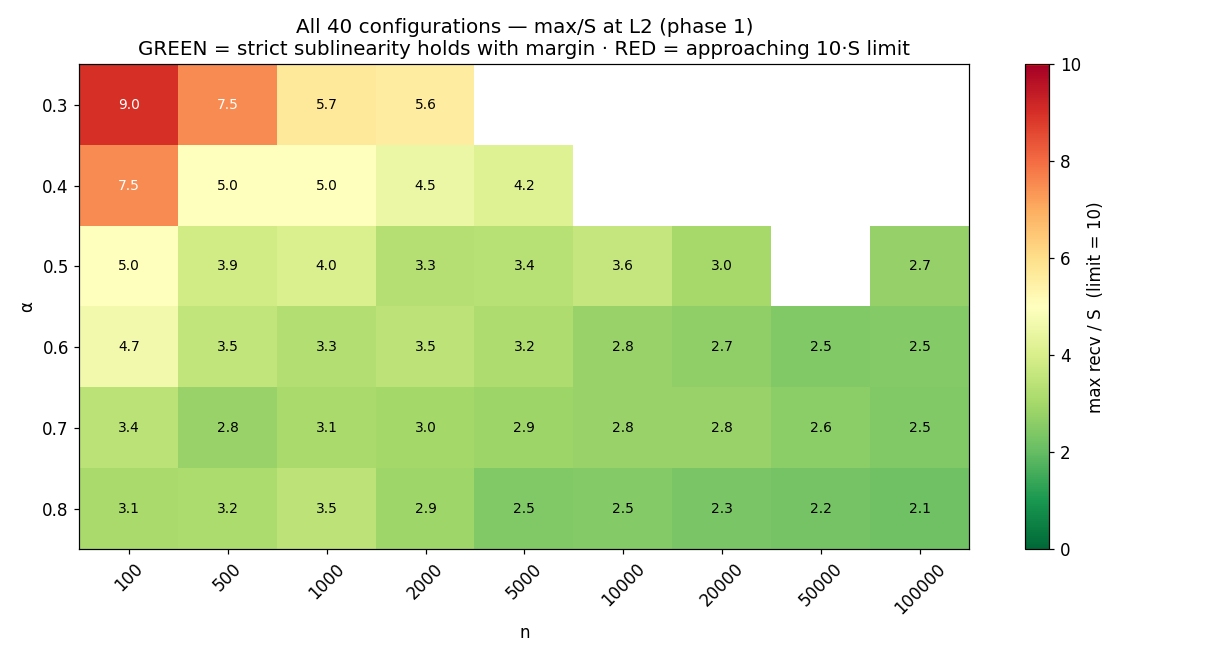
\includegraphics[width=0.95\textwidth]{plots/8_grid_overview.png}
\caption{Maximum recv per machine at Level 2, normalized by $S$, for every
$(n, \alpha)$ tested. The cell colors range from green (well within the
$10 \cdot S$ limit) to red (approaching the limit). No cell exceeds the
limit; the worst case is $9.0 \cdot S$ at $n = 100, \alpha = 0.3$, and
most cells sit between $2$ and $4 \cdot S$.}
\label{fig:grid}
\end{figure}

Figure~\ref{fig:grid} is the headline result. Three patterns emerge:
\begin{enumerate}[topsep=2pt, itemsep=2pt, leftmargin=*]
    \item No configuration exceeds the $10 \cdot S$ recv limit.
    \item For fixed $\alpha$, max/$S$ decreases as $n$ grows --- the
          Chernoff concentration tightens as $\mu$ grows.
    \item For fixed $n$, max/$S$ decreases as $\alpha$ grows --- larger
          $S$ also tightens concentration.
\end{enumerate}

\subsection{Per-level load distribution}

\begin{figure}[h]
\centering
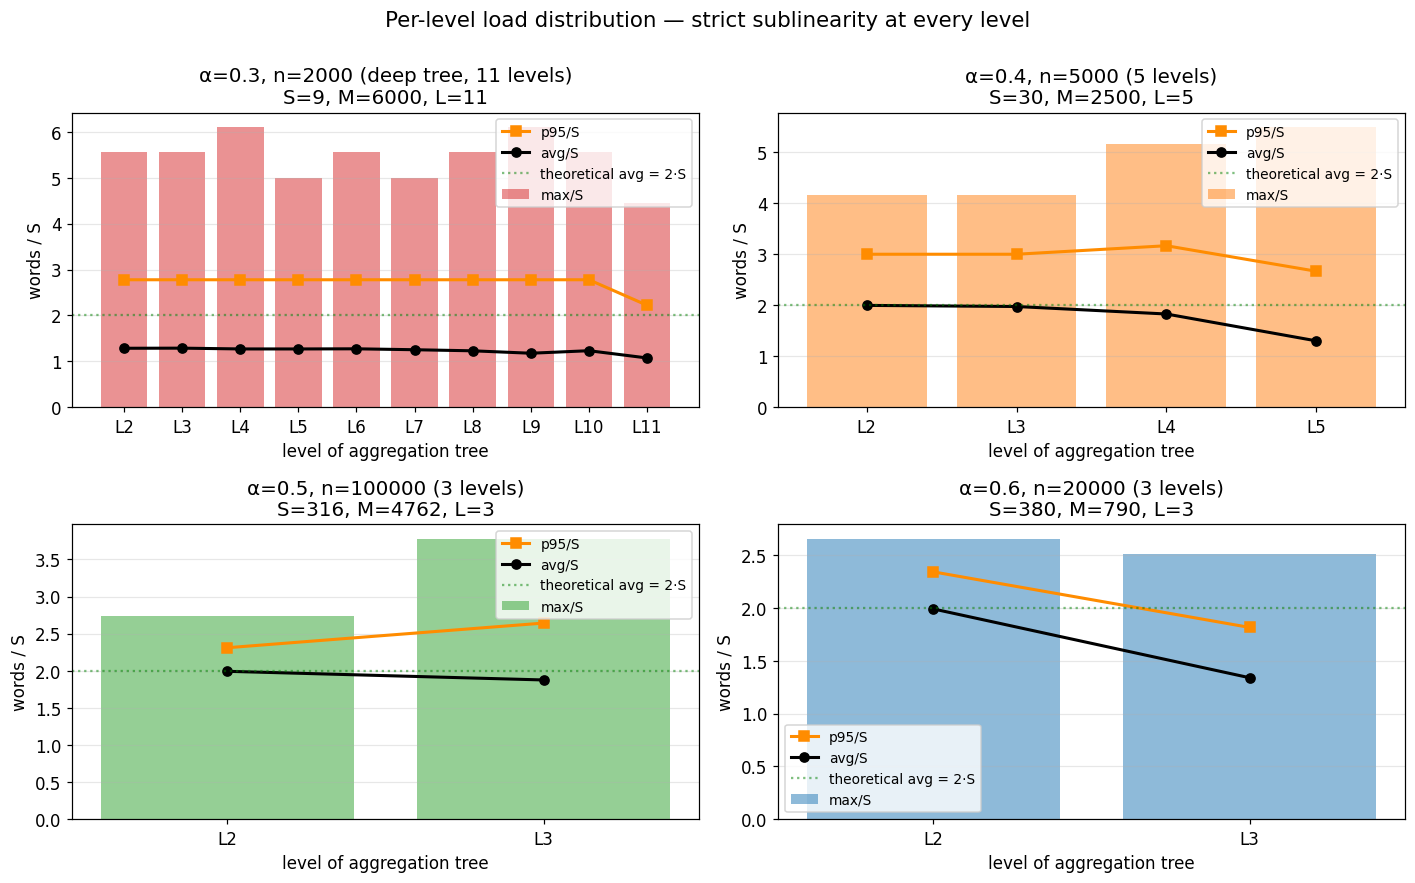
\includegraphics[width=0.95\textwidth]{plots/5_per_level_load.png}
\caption{Per-level recv distribution for four representative cases.
Each panel shows max/$S$ (bar), p95/$S$ (orange), and avg/$S$ (black) for
every level of the aggregation tree. The dashed green line marks the
theoretical avg = $2 \cdot S$ from the data-driven invariant. In every
case avg matches theory ($\le 2 \cdot S$), p95 is $\le 3 \cdot S$, and
max is $\le 6 \cdot S$.}
\label{fig:per-level}
\end{figure}

Figure~\ref{fig:per-level} shows that load is distributed uniformly across
levels (within concentration limits), not concentrated at the top. The
top-left panel ($n = 2000, \alpha = 0.3$, 11-level tree) is the most
striking: even with 10 communication levels, max/$S$ stays $\le 6$
throughout.

\subsection{Correctness and round count}

All 40 full-mode runs produce MSTs whose weight matches Kruskal's reference
exactly. Phase counts range from $21$ to $34$, matching the predicted
$\log_{4/3}(n)$ bound. Total round counts range from $84$ (small $n$,
large $\alpha$) to $1012$ (large $n$, small $\alpha$), consistent with
$O(\log n / \alpha)$. No sub-rounds were triggered; the $10 \cdot S$ recv
limit was sufficient at every step.

% ─────────────────────────────────────────────────────────────────────────
% 6. DISCUSSION & FUTURE WORK
% ─────────────────────────────────────────────────────────────────────────
\section{Discussion and Future Work}

\subsection{What the data supports vs.\ what remains untested}

The grid covers $\alpha \in [0.3, 0.8]$ and $n \in [100, 100{,}000]$.
Within this range:
\begin{itemize}[topsep=2pt, itemsep=2pt, leftmargin=*]
    \item Strict sublinearity holds with margin everywhere.
    \item The data-driven invariant matches theory tightly.
    \item Chernoff concentration tightens with $S$ as predicted.
    \item MST correctness in every case.
\end{itemize}
Untested: $\alpha < 0.3$ (very small $S$, harder Chernoff regime);
$n > 100{,}000$ at $\alpha \le 0.4$ (Python OOM); non-random graphs.

\subsection{Python as a bottleneck}

Each Python \texttt{Machine} instance carries $\approx 1.5$ KB of overhead
before holding any data. At $n = 10^5, \alpha = 0.3$ we have
$M \cdot L \approx 340{,}000$ machines, exceeding available memory.
A C++/Rust port (per-machine $\approx 100$ bytes) would lift this ceiling
by roughly $15\times$ and make $n = 10^6$ feasible.

\subsection{Where the paper's analysis is asymptotic}

The exercise sheet's Lemma~4 bounds expected indegree by $S/2$ under
$\alpha > 1/2$ and $S \ge 16$. In our regime ($\alpha < 0.5$, $S$ small)
the paper's \textit{constant} ($1/2$) does not hold, though its
\textit{asymptotic} claim ($O(S)$) does. Our maxima are bounded by
$O(\sqrt{\log n})$-factor above the data-driven average, in line with
Chernoff predictions.

\subsection{Future work}

\begin{itemize}[topsep=2pt, itemsep=2pt, leftmargin=*]
    \item C++/Rust port to extend testing to $n \ge 10^6$ at low
          $\alpha$.
    \item Empirical comparison of branching factor $b = \sqrt{S}$ vs.\
          the paper's $b = S/4$. The former is the smallest $b$ for which
          the random-argument bound on indegree holds at every level.
    \item Mitigation of top-level concentration via $R(x, L_\text{top})
          \ge 2$ (instead of forcing $= 1$).
    \item Testing on real-world (non-random) graphs.
\end{itemize}

% ─────────────────────────────────────────────────────────────────────────
% 7. CONCLUSION
% ─────────────────────────────────────────────────────────────────────────
\section{Conclusion}

This work delivers a complete and empirically verified implementation of
Bor\r{u}vka's MST algorithm in the sublinear MPC regime. Four implementation
choices depart from the paper of Bamberger--Kuhn:
\begin{enumerate}[topsep=2pt, itemsep=2pt, leftmargin=*]
    \item depth uncapped to natural $\lceil \log_{S/4}(m) \rceil$;
    \item direct top$\to$L1 downward in one round;
    \item step-doubling $k$-ary distributed termination;
    \item strict $O(S)$ hard-checked per-machine limits.
\end{enumerate}
Across 44 configurations ($n$ up to $100{,}000$, $\alpha \in [0.3, 0.8]$)
the simulator achieves zero violations, zero sub-rounds, and correct MSTs.
Max recv stays bounded by $9 \cdot S$ in the worst case (small $n$, small
$\alpha$) and drops toward $2 \cdot S$ in the asymptotic regime --- exactly
what Chernoff predicts.

% ─────────────────────────────────────────────────────────────────────────
% REFERENCES
% ─────────────────────────────────────────────────────────────────────────
\begin{thebibliography}{9}

\bibitem{exercise12}
P.~Bamberger and F.~Kuhn.
\textit{Distributed Systems, Exercise Sheet 12 --- Bor\r{u}vka's MST
Algorithm in the Strongly Sublinear MPC Model.}
University of Freiburg, Summer Term 2020.

\bibitem{ghs}
R.~G. Gallager, P.~A. Humblet, P.~M. Spira.
\textit{A Distributed Algorithm for Minimum-Weight Spanning Trees.}
ACM TOPLAS 5(1), 1983.

\bibitem{karloff}
H.~J. Karloff, S.~Suri, S.~Vassilvitskii.
\textit{A Model of Computation for MapReduce.}
SODA 2010.

\bibitem{ghaffari}
M.~Ghaffari.
\textit{Massively Parallel Algorithms.}
Lecture notes, ETH Z\"urich, 2019.

\end{thebibliography}

\end{document}
